%%%%%%%%%%%%%%%%%%%%%%%%%%%%%%%%%%%%%%%%%%%%%%%%%%%%%%%%%%%%%%%%%%%%%%
%     File: ExtendedAbstract_backg.tex                               %
%     Tex Master: ExtendedAbstract.tex                               %
%%%%%%%%%%%%%%%%%%%%%%%%%%%%%%%%%%%%%%%%%%%%%%%%%%%%%%%%%%%%%%%%%%%%%%

\section{Related Work}
\label{sec:related}

Our work builds upon two primary research areas: the development of comprehensive aerial image datasets that capture the unique characteristics of overhead imagery, and the evolution of specialized architectures for referring remote sensing image segmentation. This section examines the progression from traditional semantic and instance segmentation datasets to modern referring segmentation benchmarks, and reviews the architectural innovations that have advanced the state of the art in language-driven aerial image analysis.

\subsection{Aerial Image Datasets}

The development of aerial image understanding has been significantly advanced by the creation of comprehensive datasets that capture the unique characteristics of overhead imagery. Traditional aerial datasets initially focused on semantic and instance segmentation tasks, with iSAID (instance segmentation in Aerial Images Dataset) providing fine-grained instance-level annotations for objects in high-resolution satellite images, and LoveDA (Land-cOVEr Domain Adaptive semantic segmentation) offering semantic segmentation annotations across diverse geographical regions with domain adaptation challenges.

The emergence of referring segmentation in aerial imagery marked a significant evolution in dataset development. RefSegRS introduced the first referring remote sensing image segmentation dataset, establishing the foundation for language-driven segmentation in overhead imagery. This pioneering work demonstrated the feasibility of combining natural language descriptions with aerial image segmentation, opening new research directions in the remote sensing community.

Building upon this foundation, RRSIS-D (Referring Remote Sensing Image Segmentation Dataset) expanded the scope and complexity of referring segmentation in aerial domains, providing more comprehensive annotations and challenging scenarios that better reflect real-world applications. More recently, NWPU-Refer has further advanced the field by introducing additional complexity and scale, contributing to the growing ecosystem of referring segmentation datasets for aerial imagery. These datasets collectively demonstrate the increasing recognition of the importance of natural language interfaces for aerial image analysis tasks.

\subsection{Architectures for RRSIS}

The development of specialized architectures for referring remote sensing image segmentation has evolved alongside the dataset contributions, with each major dataset introducing novel architectural innovations. The initial RefSegRS work established fundamental approaches for combining language understanding with aerial image segmentation, while RRSIS-D introduced refinements that better addressed the unique challenges of overhead imagery, including varying scales and specialized object categories.

The NWPU-Refer contribution further advanced architectural design by incorporating more sophisticated attention mechanisms and multi-scale processing capabilities tailored to the characteristics of aerial scenes. Each of these works has contributed distinct architectural components that have collectively advanced the state of the art in referring segmentation for remote sensing applications.

Among these developments, RSRefSeg has emerged as a particularly robust architecture that leverages both SigLIP and SAM as its foundational backbones. As illustrated in Figure \ref{fig:rsrefseg_architecture}, RSRefSeg achieves state-of-the-art performance when trained and evaluated on RRSIS-D, establishing it as a solid foundational architecture for work in this area. The architecture employs a dual-encoder approach utilizing SigLIP for text and image feature extraction, followed by SAM for high-quality segmentation mask generation.

The RSRefSeg architecture consists of several key components that work in concert to achieve robust referring segmentation. The SigLIP encoders process both natural language descriptions and visual content, while specialized prompter networks serve as adapters that transform SigLIP features into SAM-compatible prompt embeddings. The system leverages local and global activation mechanisms for fine-grained text-image alignment, and employs parameter-efficient LoRA fine-tuning to maintain the strong pre-trained capabilities of both foundation models while enabling adaptation to the aerial domain.

\begin{figure*}[t]
\centering
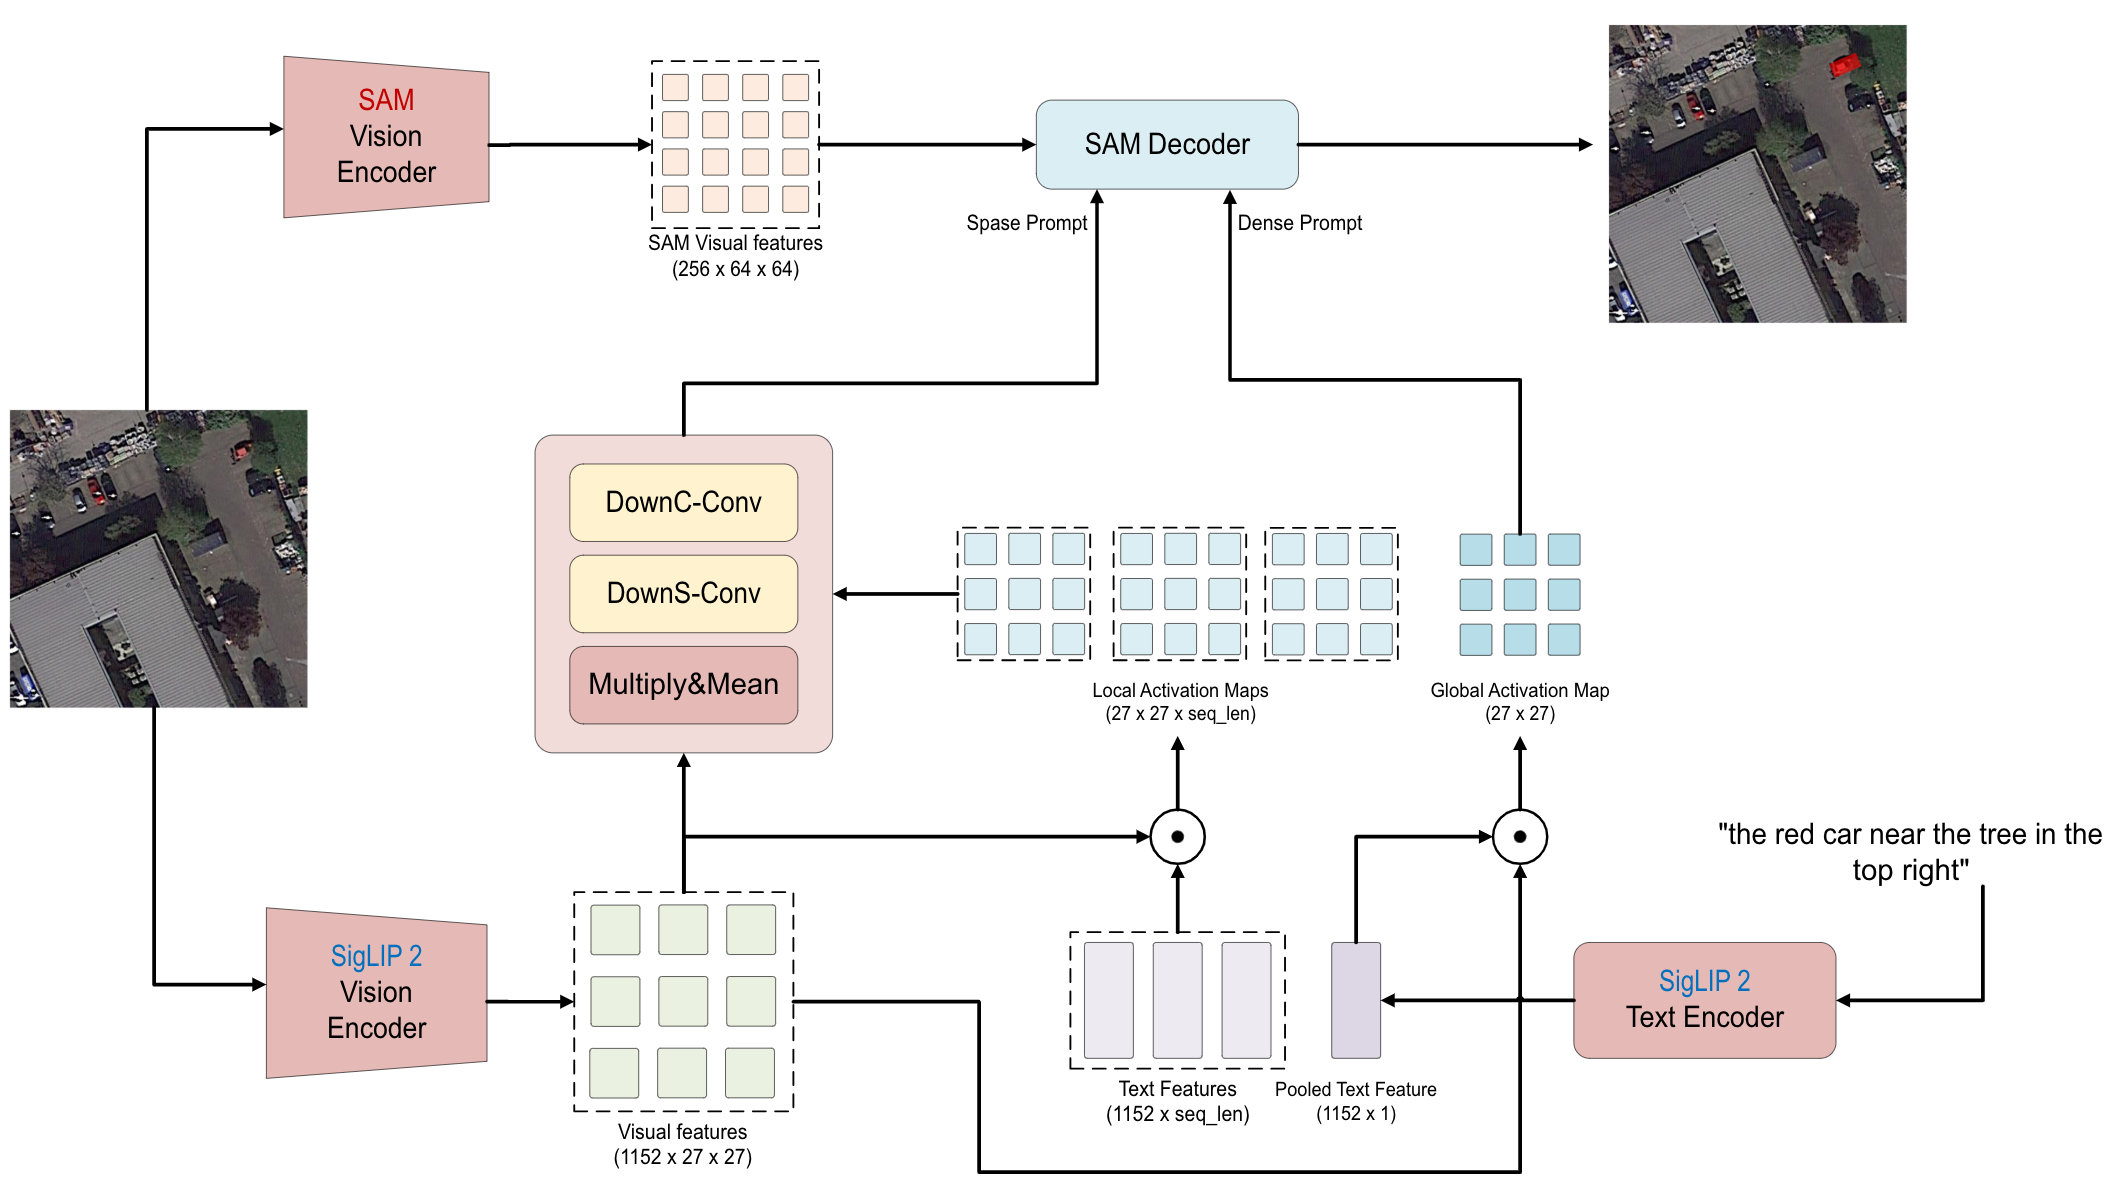
\includegraphics[width=0.85\textwidth]{./images/rsrefseg.png}
\caption{RSRefSeg architecture combining SigLIP text-image encoding with SAM mask generation for referring segmentation tasks. The architecture employs dual encoders with specialized prompter networks to bridge vision-language understanding with precise segmentation.}
\label{fig:rsrefseg_architecture}
\end{figure*}

